\documentclass[beamer,dvipsnames]{standalone}

\usepackage{tikz}
\usetikzlibrary{arrows}
\usetikzlibrary{positioning}
%\usetikzlibrary{positioning,decorations.pathreplacing,fit}
\usetikzlibrary{decorations.markings,arrows.meta}

\usepackage{bm}

\providecommand{\adlog}{\textcolor{red}{a}}
\providecommand{\bdlog}{\textcolor{blue}{b}}
\providecommand{\getsr}{\overset{\$}{\gets}}
\providecommand{\edloga}{\textcolor{red}{a'}}
\providecommand{\edlogb}{\textcolor{blue}{b'}}


\begin{document}

\begin{standaloneframe}

\resizebox{1\textwidth}{!}{

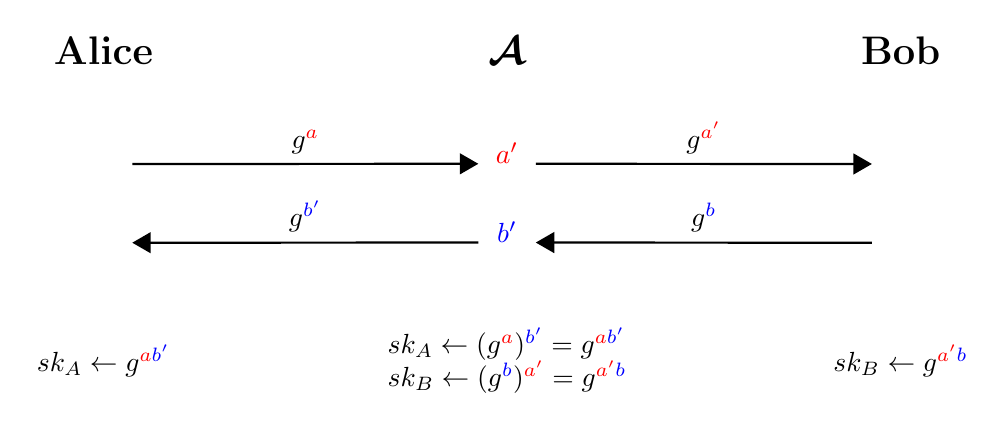
\begin{tikzpicture}[
		>=triangle 60,
	   	every path/.style={
	   		thick
	   	}
	]
	
	
	\node (client) {\Large\bfseries Alice};
	\node[right=4cm of client] (E) {\Large$\bm{\mathcal{A}}$};
	\node[right=4cm of E] (server) {\Large\bfseries Bob};
	

	\newcommand*{\MsgSpace}{0.5}
	\foreach \i in {1, ..., 7} {
		\node[below = \i * \MsgSpace of client,inner xsep=10pt] (c\i) {};
		\node[below = \i * \MsgSpace of E,inner xsep=10pt] (e\i) {};
		\node[below = \i * \MsgSpace of server,inner xsep=10pt] (s\i) {};
	}
	
	
	\draw[->] (c2.east) -- node[above] (M1) {$g^{\adlog}$} (e2.west);
	
	\uncover<2->{
		\node at (e2.north) {$\edloga$};
		\draw[->] (e2.east) -- node[above] (M1) {$g^{\edloga}$} (s2.west);
	}
	
	\uncover<3->{
		\draw[<-] (e4.east) -- node[above] (M2) {$g^{\bdlog}$} (s4.west);
	}
	
	\uncover<4->{
		\node at (e4.north) {$\edlogb$};
		\draw[<-] (c4.east) -- node[above] (M2) {$g^{\edlogb}$} (e4.west);	
	}
	
	\uncover<5->{
		\node[] at (c7) {$sk_A \gets g^{\adlog\edlogb}$}; 	
	}
	
	\uncover<6->{
		\node[] at (s7) {$sk_B \gets  g^{\edloga\bdlog}$}; 	
	}

	
	\uncover<7>{
		\node[align=left] at (e7) {
			$sk_A \gets (g^{\adlog})^{\edlogb} = g^{\adlog\edlogb}$\\
			$sk_B \gets (g^{\bdlog})^{\edloga} = g^{\edloga\bdlog}$
		};
	}
	
	
\end{tikzpicture}

}

\end{standaloneframe}

\end{document}